It is unlikely to have a model perform as one expects the first time. There are
therefore a few techniques for optimizing the performance. It should be noted
that much of the discussion here and in Section \ref{sec:valid} focuses on the
diagnostics aspect rather than the validation aspect of these techniques. In
practice, these are used for both purposes: diagnosing fitness problems and
proving good fitness.  But this work uses a formal comparison of model
performance for validation, introduced and detailed in Sections
\ref{sec:invcompare} and \ref{sec:modelcompare}, respectively. 

However, there is a risk associated with better prediction after using
optimization tools.  The increase in performance from over-optimization could
be linked to the training set performance and might not generalize outside of
the specific type of input data used.  A workaround for this scenario is to
obtain more data for the set or to obtain a completely different data set
altogether. 

\subsubsection{Training Set Size}

The first diagnostic plot for optimizing the model performance is called a
\textit{learning curve}, which provides information about the bias-variance
tradeoff with respect to the data set size. More specifically, learning curves
compare the training and \gls{CV} errors to the size of the training
set (i.e., number of instances in the training set). This is done by randomly
selecting a percentage of the the training set, inputting that into a
statistical learner, and tabulating the error of the learned model. 

Typically, a learning curve will look somewhat like one of the three examples
in Figure \ref{fig:learning}\footnote{These schematics are based on hand-drawn
diagrams by Ritchie Ng on http://www.ritchieng.com/applying-machine-learning/}.
A learning curve tests the model for high bias or high variance, which can
correspond to an under- or overfit model, respectively. 

\begin{figure}[!hp]
  \centering
  \begin{subfigure}[h]{0.65\linewidth}
    \centering
    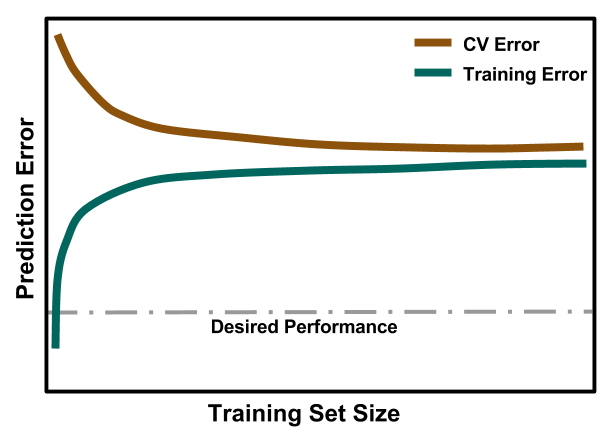
\includegraphics[width=\linewidth]{./chapters/litrev/LearningCurve-bias.png}
    \caption{High bias}
    \label{fig:bias}
  \end{subfigure}
  \begin{subfigure}[h]{0.65\linewidth}
    \centering
    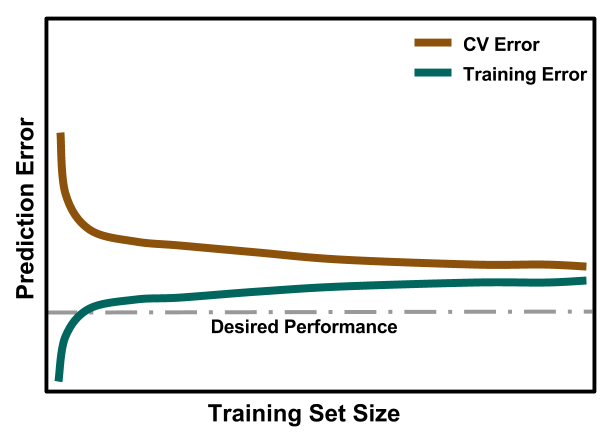
\includegraphics[width=\linewidth]{./chapters/litrev/LearningCurve-ideal.png}
    \caption{Ideal}
    \label{fig:ideal}
  \end{subfigure}
  \begin{subfigure}[h]{0.65\linewidth}
    \centering
    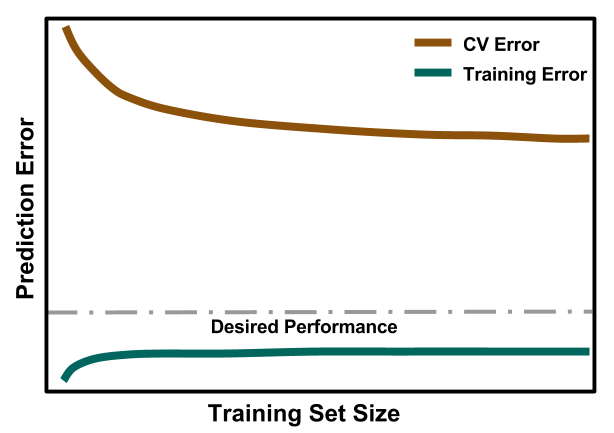
\includegraphics[width=\linewidth]{./chapters/litrev/LearningCurve-variance.png}
    \caption{High variance}
    \label{fig:variance}
  \end{subfigure}
  \caption{Learning Curves for Three Training Scenarios}
  \label{fig:learning}
\end{figure}

Figure \ref{fig:bias} suggests underfitting because the model is missing
important features in the data. It is characterized by a small gap between the
curves but high overall errors. The \gls{CV} error remains consistently
high and the training error increases drastically with increasing data, since
it is not generalizing well. 

Figure \ref{fig:variance} suggests overfitting because the model has too much
sensitivity to variations in the data. It is characterized by a very large gap
between the curves. It has an extremely low training error, as it has taken
into account every detail of the training set, but a high \gls{CV}
error because it cannot generalize beyond the testing set. 

Figure \ref{fig:ideal} is an example of a more ideal model fit. It is
characterized by a small gap between the two errors, and they are at a
reasonable level with respect to the desired performance.  The training error
should increase with respect to the training set size due to a larger amount of
bias (preventing overfitting). However, the \gls{CV} error should decrease
quickly with respect to the training set size due to being close to the minimum
of the bias-variance tradeoff. 

The training set size must be large and diverse enough to be considered
\gls{i.i.d.} because most \gls{ML} algorithms are developed upon this
assumption. Sometimes this is not possible, and the training data are skewed,
i.e., a portion of the data is over-represented. This must be handled
explicitly, but since each algorithm handles skewed data differently, it is
currently beyond the scope of this work. 

\subsubsection{Model Complexity}

After ensuring the appropriate training set size is selected, the models must
be further optimized using \textit{validation curves}.  These provide
information on the bias-variance tradeoff with respect to model complexity. Two
main tuneable factors affecting model complexity can cause the model to be
under- or overfit to the data: number of features in the data set and algorithm
parameters that control the regularization.

\begin{figure}[!htb]
  \centering
  \makebox[\textwidth][c]{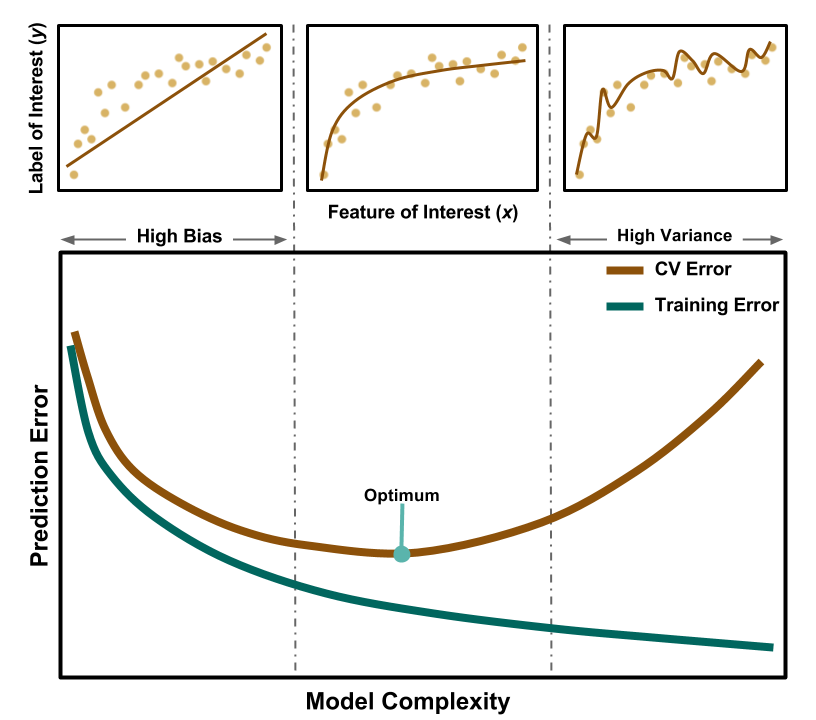
\includegraphics[width=1.2\textwidth]{./chapters/litrev/ValidationCurve.png}}
  \caption{Validation Curve with Different Model Fits}
  \label{fig:validation}
\end{figure}

Figure \ref{fig:validation} adapted from Ref. \cite{elements_stats} shows the
optimum as the minimum of the \gls{CV} error curve in the main (bottom)
plot. There is some gap between it and the training error, much larger than the
left side of the plot and much smaller than the right.  The top-middle plot is
a simplified visualization of an approximately well-fit model.  The left region
is marked by both errors being quite high, and above is an  illustration of how
an underfit plot (high bias) could provide high errors. The right region shows
the training error being quite low but the \gls{CV} error being high.
The diagram differing options with how to adjust to skewed training sets
\cite{scikit}.  above shows that it is obvious how the training error would be
negligible, but generalizing beyond that probably will not yield accurate
results. 

In practice, plotting learning and validation curves can be iterative. But as
previously mentioned, too many optimizations will result in a poorly performing
model when exposed to data outside of the training set.

\subsubsection{Comparison of Models}
\label{sec:invcompare}

In addition to evaluating a single learned model, it is beneficial to compare
models. Moreover, there are potential degeneracies in the solution space. This
is because most inverse problems are \textit{ill-posed}, because the solution
is not guaranteed to be unique \cite{skutnik_2016}.  Evaluating not only the
solution, but the confidence in the solution, is therefore prudent.

Both solution uncertainty and model comparison can be done using Bayesian
inference as discussed in Section \ref{sec:inverse}.  Equations \ref{eq:bayes}
and \ref{eq:bayes_words} show that there are three values to obtain to
calculate a posterior probability, i.e., the probability of a parameter
estimated from an \gls{ML} model being correct: likelihood, prior
probability, and marginal likelihood.  Comparing posterior probabilities among
different models reveal the most probable correct answer, i.e., the highest
posterior probability.  \cite{inverse_theory, gentle_bayes} Each of these
values are explained futher below.

The posterior probability represents the solution to an \textit{inverse}
problem, where model parameters are predicted from some given measurement
values. It is not directly computable and thus the remaining probabilities
discussed below indirectly allow its computation.  In this context, it is the
probability that a predicted reactor parameter from a chosen \gls{ML}
algorithm is correct given input based on an \gls{SNF} recipe.  For example, it
is the probability that a plutonium-239 concentration of $y\%$ is attributed to
a uranium oxide fuel in a \gls{BWR} with a burnup of $x\ GWd/MTU$.  

\begin{table}[!hp]
  \centering
  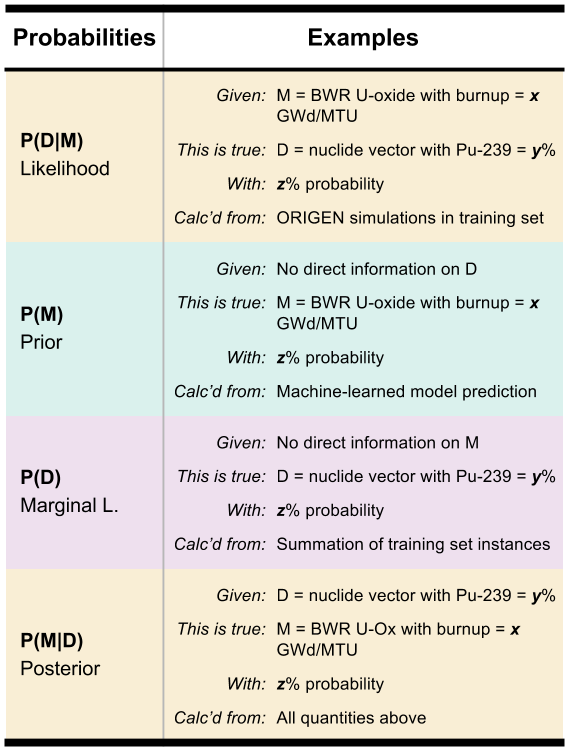
\includegraphics[width=\linewidth]{./chapters/litrev/bayes.png}
  \caption{Summary of Bayes Theorem Components}
  \label{tbl:bayes}
\end{table}

The prior probability represents the solution to a \textit{forward} problem,
where measurement values are predicted from some given model parameters.  In
this context, this is calculated from the instances in the training data set.
The likelihood is the probability that the output \gls{SNF} composition of a
simulation is correct given the input of reactor operation parameters.  In
practice, it will be calculated from a large number of forward simulations
using \gls{ORIGEN}, i.e., the training data set. For example, this would be the
probability that uranium oxide fuel from a \gls{BWR} having a burnup of $x\
GWd/MTU$ contains $y\%$ of plutonium-239.

The likelihood represents the spread of plausible \textit{model parameters}, so
it is a hypothesis based on the breadth of the model space with no evidence
provided.  In other words, it is given by model parametertization from a number
of potential sources.  One method is expert-elicited values.  Another is a
predicted model from some established theory or previously known relationship,
e.g., empirical relations between isotopic ratios and certain reactor
parameters or a direct calculation of the reactor parameters. In this context,
it is obtained from the estimated model parameters from a given statistical
model.  For example, it is the probability that a model from \gls{SVR} predicts
a burnup of $x\ GWd/MTU$ for uranium oxide fuel from a \gls{BWR} with no other
direct measurements provided.

The marginal likelihood represents the spread of plausible
\textit{measurements}, so it is based on the breath of the data space with no
model-based information provided.  In practice, however, it is calculated by
summing the joint probabilities of all possible model parameter hypotheses and
measurements. This in essence provides a normalization constant for the Bayes'
equation.  Thus, the marginal likelihood is only needed for absolute posterior
probability calculations; it does not affect the relative probabilities, which
are all that is needed for model comparison. \cite{inverse_theory,
bayes_compare}

For reference, Table \ref{tbl:bayes} is a summary of the Bayes' theorem
components described above as related to this work. In the table, \textbf{P} is
a probability, \textbf{D} is a set of measurements (i.e., data), and \textbf{M}
is a set of model parameters. The examples used in the discussion above are
reiterated here.

